\subsection{Data conversion architecture}

OpenEHR integration information model architecture, shown in \ref{fig:data_conversion_architecture}, is designed for inherited integration situations.

\begin{figure}[h]
  \centering
  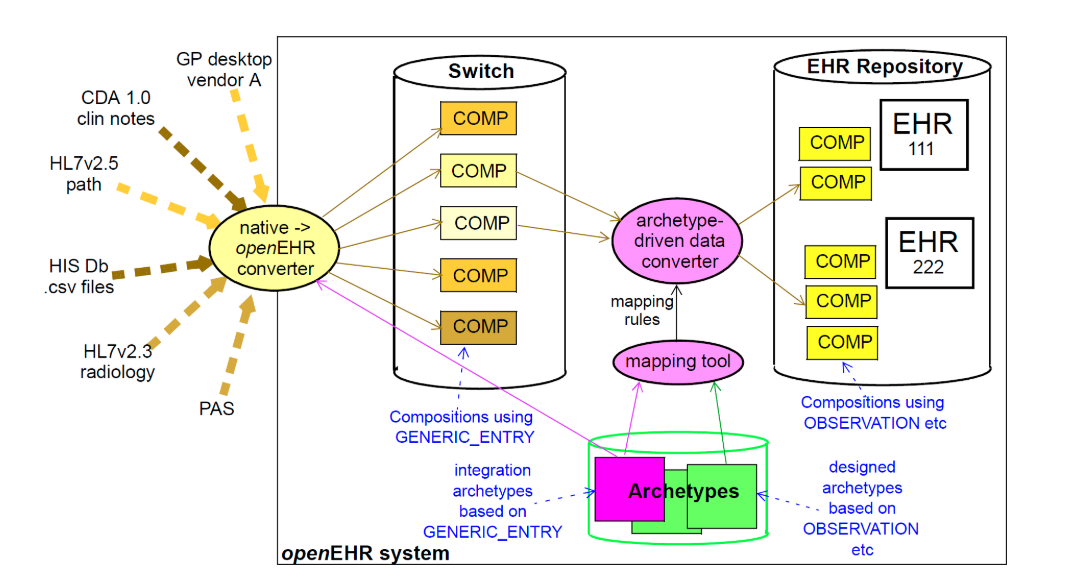
\includegraphics[scale=0.4]{./images/data_conversion_architecture}
  \caption{Data integration in openEHR (Source: extracted from \cite{openEHR}).}
  \label{fig:data_conversion_architecture}
\end{figure}

Design is based on a clear separation of the syntactic and semantic transformation  required in imported data in openEHR. Syntactic transformation converts data from their original syntactic format into openEHR reference model structures, whose logical and semantic structures are controlled by integration archetypes that imitate the data's original design. As a result of the conversion, data can be processed in openEHR. The semantic transformation converts imported data to clinical archetypes.

The openEHR elements that make this transformation possible are:
\begin{itemize}
  \item GENERIC\_ENTRY class which is used to create intermediate representations of data from sources that otherwise won't adjust to openEHR classes;
  \item integration archetypes defined using GENERIC\_EN\-TRY class;
  \item clinical archetypes designed from ENTRY sub classes;
  \item semantic transformation rules between integration archetypes and clinical archetypes.
\end{itemize}
